\documentclass[12pt, letterpaper, titlepage]{article}

\usepackage[utf8]{inputenc}
\usepackage{hyperref}
\usepackage{listings}
\usepackage{graphicx}

\begin{document}

% Create a title page
\begin{titlepage}
	\centering
	{\scshape\LARGE BITS Pilani, Goa Campus \par}
	\vspace{1cm}
	{\scshape\Large Network Programming Project\par}
	\vspace{2cm}
	{\large\textit{Utkarsh Maheshwari\\2015A7PS022G}}

	% Fill page with blank space
	\vfill
	supervised by\par
	Mr.~Mahadev A.~Gawas
	\vfill

    % Bottom of the page
    {\large September, 2017}
\end{titlepage}

% Show table of contents and end page
\tableofcontents
\newpage


\section{Abstract}

    \paragraph{}
    The project aims to create a way for \textbf{Android} phones and
    \textbf{GNU/Linux} laptops to connect and communicate with each other on a
    local area network, be it wired or wireless.

    \paragraph{}
    The project is expected to send all Android notifications to the laptop and
    all laptop notifications to the phone. The project can also be extended to
    provide support to get tty access on a phone that is connected to the
    laptop providing (virtually) unlimited functionality.


\section{Learning Scope}

    \paragraph{}
    This project can provide a lot of learning opportunities including but not
    limited to:
    \begin{itemize}
        \item{How to connect two nodes on a local area network}
        \item{How to send data targetting a specific node}
        \item{How to implement various authentication/authorization and
            encryption protocols}
        \item{How to implement network security}
        \item{How to create user space applications which can communicate with
            other applications running on different architecture}
        \item{How to select between different types of protocols based on the
            type of data to be sent}
    \end{itemize}


\newpage
\section{Project Features}

    \paragraph{Security}
    Security is the top priority of the project keeping in mind the proper
    protocols and methods. The project is expected to eventually implement the
    most popular and secure encryption and authorization protocols.

    \paragraph{Speed}
    The application will be written in \textbf{pure C} for linux and use the
    system libraries ensuring greater speed than it's equivalent in Python or
    Java.  Due to being compiled to machine code and running in the userspace
    without any virtual machine, this can feature \textbf{faster} execution and
    weighs \textbf{lesser} on the CPU resources.

    \paragraph{No internet costs}
    The application is expected to allow devices on the same local area network
    to communicate making it both secure and less resource heavy, requiring
    \textbf{no internet}.


\section{Extension}

    \paragraph{}
    Although the functionality for this project is limited due to the short
    duration of the course, it can eventually provide the following features if
    continued:
    \begin{itemize}
        \item{Mobile telephony on laptop}
        \item{Using phone as a virtual mouse/keyboard}
        \item{File transfer}
        \item{Using laptop speakers for playing music via phone or vice versa}
    \end{itemize}


\newpage
\section{Similar Projects}

    \paragraph{}
    These projects too aim for providing this functionality although only
    KDEConnect can provide the same without the use of internet.
    \begin{itemize}
        \item{\
            \href{https://community.kde.org/KDEConnect}{KDEConnect}
            \begin{figure}[h!]
                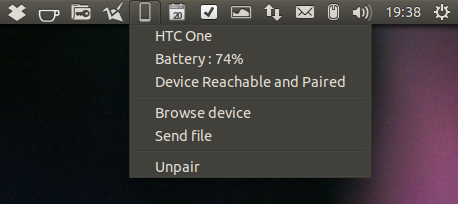
\includegraphics[width=0.75\textwidth]{kdeconnect.png}
                \centering
                \caption{KDEConnect example}
            \end{figure}
        }
        \item{\
            \href{https://www.pushbullet.com/}{Pushbullet}
            \begin{figure}[h!]
                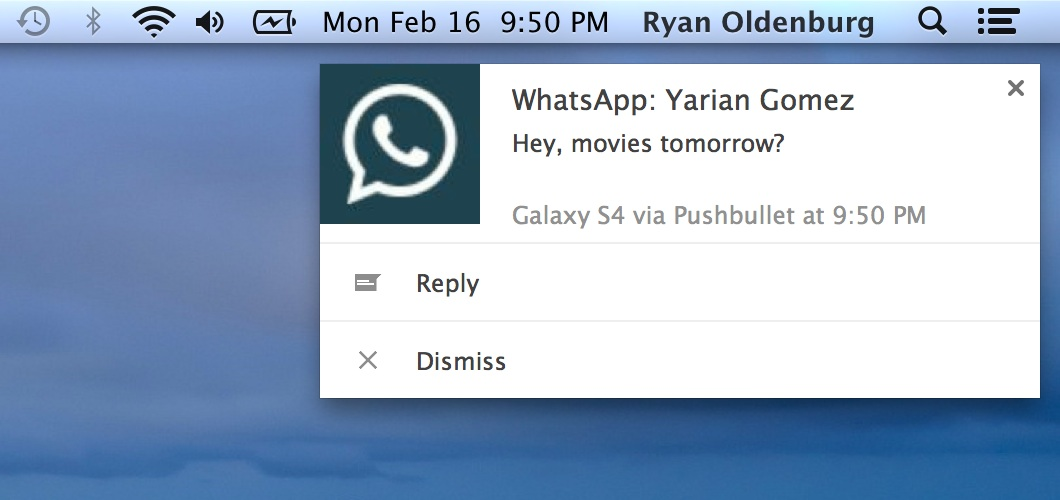
\includegraphics[width=0.75\textwidth]{pushbullet.jpg}
                \centering
                \caption{Pushbullet example}
            \end{figure}
        }
        \item{\href{https://ifttt.com/}{IFTTT}}
    \end{itemize}

\end{document}
